\documentclass[sigconf]{acmart}
\settopmatter{printacmref=false,printccs=false,printfolios=false}
\usepackage{tikz}\usetikzlibrary{positioning}\usepackage{pifont}
\pagestyle{empty}
\begin{document}
\thispagestyle{empty}
\noindent
  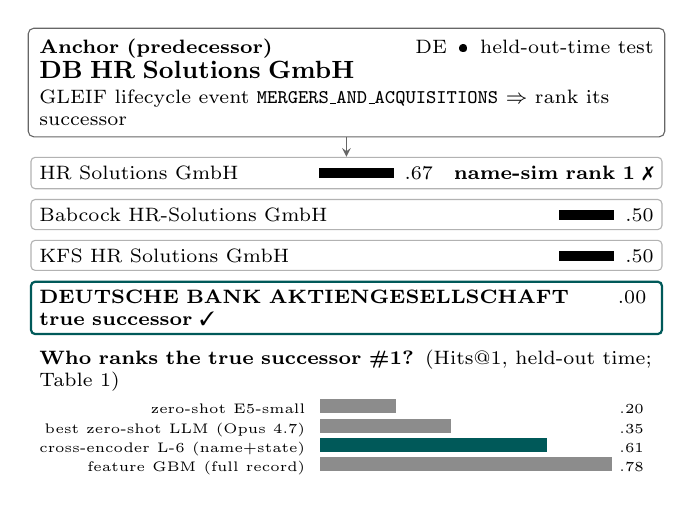
\begin{tikzpicture}[
      every node/.style={font=\scriptsize},
      card/.style={draw=black!60, rounded corners=2pt, inner sep=4pt,
                   text width=222pt, align=left},
      cand/.style={draw=black!30, rounded corners=1.5pt, inner sep=3pt,
                   text width=222pt, align=left},
      gold/.style={cand, draw=teal!70!black, thick},
      node distance=3.5pt
  ]
  \node[card] (a) {\textbf{Anchor (predecessor)} \hfill
      DE \,\textbullet\, held-out-time test\\[1pt]
      {\small\textbf{DB HR Solutions GmbH}}\\[1pt]
      GLEIF lifecycle event \texttt{MERGERS\_AND\_ACQUISITIONS}
      $\Rightarrow$ rank its successor};
  \node[cand, below=7pt of a] (c1) {HR Solutions GmbH \hfill
      \rule[0.5pt]{27pt}{3.5pt}\, .67 \;
      \textbf{name-sim rank 1} \ding{55}};
  \node[cand, below=of c1] (c2) {Babcock HR-Solutions GmbH \hfill
      \rule[0.5pt]{20pt}{3.5pt}\, .50};
  \node[cand, below=of c2] (c3) {KFS HR Solutions GmbH \hfill
      \rule[0.5pt]{20pt}{3.5pt}\, .50};
  \node[gold, below=of c3] (c4) {\textbf{DEUTSCHE BANK
      AKTIENGESELLSCHAFT} \hfill .00 \;
      \textbf{true successor} \ding{51}};
  \draw[-stealth, black!60] (a.south) -- (c1.north);
  \node[below=5pt of c4, text width=222pt, align=left,
        inner sep=0] (bars) {%
    \scriptsize\textbf{Who ranks the true successor \#1?}
    (Hits@1, held-out time; Table~1)\\[2pt]
    \tiny
    \begin{tabular}{@{}r@{\ \ }l@{\ }r@{}}
    zero-shot E5-small &
      \textcolor{black!45}{\rule[0.2pt]{27.4pt}{5pt}} & .20\\
    best zero-shot LLM (Opus 4.7) &
      \textcolor{black!45}{\rule[0.2pt]{47.3pt}{5pt}} & .35\\
    cross-encoder L-6 (name+state) &
      \textcolor{teal!70!black}{\rule[0.2pt]{81.9pt}{5pt}} & .61\\
    feature GBM (full record) &
      \textcolor{black!45}{\rule[0.2pt]{105.6pt}{5pt}} & .78\\
    \end{tabular}};
  \end{tikzpicture}
\end{document}
